\section{几何}

\title[第3讲\quad 几何]{第3讲\quad 几何} 
\author{}
\date{}

\begin{frame}
    \titlepage
\end{frame}

\setcounter{framecounter}{0}

% 平面几何-直线型

\begin{frame}
    \stepcounter{framecounter}
    \frametitle{习题\theframecounter}
    \textit{在长方形 ABCD 中,P、Q 分别是 AD、BC的中点, $EM\mathop{//} NF\mathop{//} AD, AE=CF=6$, 影部分面积为 51,那么 AD 的长度为 \underline{\hbox to 20mm{}}.} 
    \begin{figure}[H] 
        \centering
        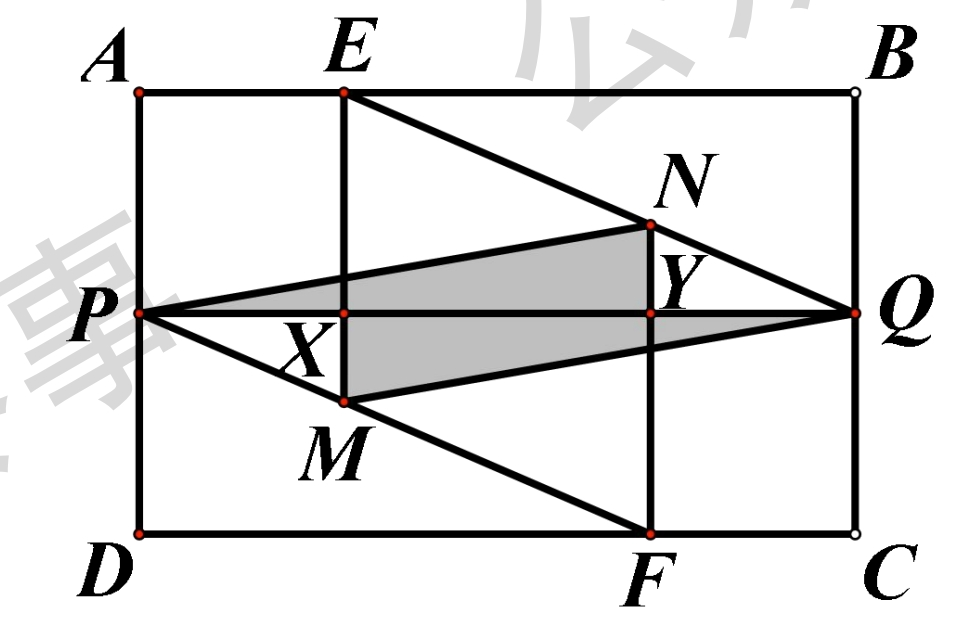
\includegraphics[width=0.4\textwidth]{./pics/Chapter_3/1.png}
    \end{figure}
    % 17
\end{frame}

\begin{frame}
    \stepcounter{framecounter}
    \frametitle{习题\theframecounter}
    \textit{如图,边长为24的大正方形被分成了五个周长相等的长方形,那么阴影长方形的面积是 \underline{\hbox to 20mm{}}.} 
    \begin{figure}[H] 
        \centering
        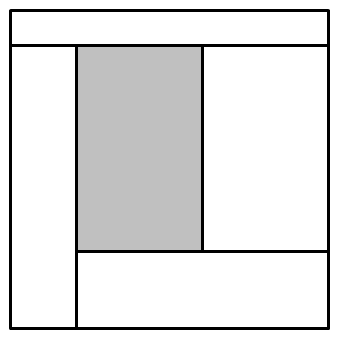
\includegraphics[width=0.4\textwidth]{./pics/Chapter_3/2.png}
    \end{figure}
    % 
\end{frame}

\begin{frame}
    \stepcounter{framecounter}
    \frametitle{习题\theframecounter}
    \textit{如图,正六边形ABCDEF中,以AB为边长向内作正方形ABGH,CG与FH交于点M.\\
    (1)如果正六边形ABCDEF的边长是20,那么三角形AFH的面积是\underline{\hbox to 20mm{}}.\\
    (2)如果正六边形ABCDEF的面积是24,那么阴影部分面积之和是\underline{\hbox to 20mm{}}.} 
    \begin{figure}[H] 
        \centering
        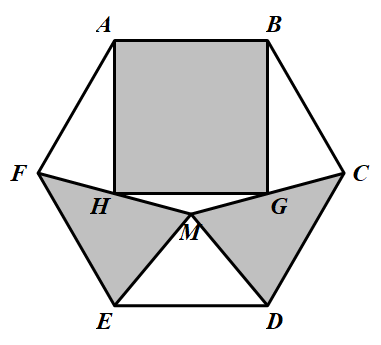
\includegraphics[width=0.4\textwidth]{./pics/Chapter_3/3.png}
    \end{figure}
    % 
\end{frame}

\begin{frame}
    \stepcounter{framecounter}
    \frametitle{习题\theframecounter}
    \textit{如图,一个大正方形被分割成了周长依次为70、80、90、100的四个小长方形;那么,其中最小的小长方形的面积是\underline{\hbox to 20mm{}}.} 
    \begin{figure}[H] 
        \centering
        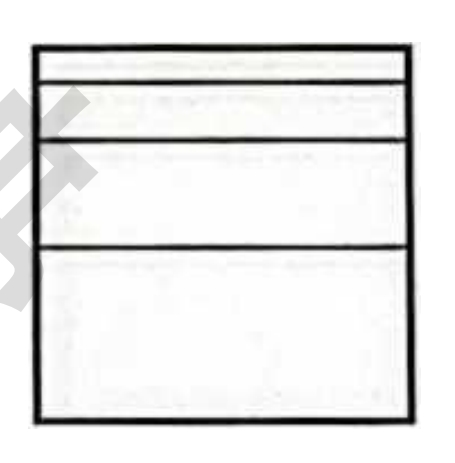
\includegraphics[width=0.4\textwidth]{./pics/Chapter_3/4.png}
    \end{figure}
    % 34
\end{frame}


\begin{frame}
    \stepcounter{framecounter}
    \frametitle{习题\theframecounter}
    \textit{两个完全一样的长方形如图摆放,如果整个图形的面积灭是 420平方厘米,那么阴影部分的面积是方厘米\underline{\hbox to 20mm{}}平方厘米.} 
    \begin{figure}[H] 
        \centering
        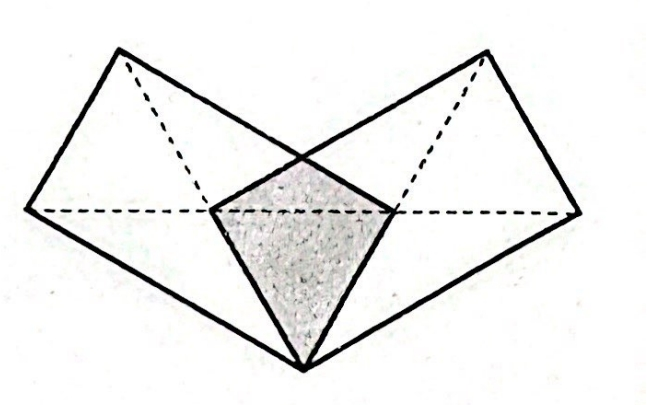
\includegraphics[width=0.4\textwidth]{./pics/Chapter_3/5.png}
    \end{figure}
    % 84
\end{frame}

% 平面几何-曲线型

% 立体几何

